\section{Related Work}

Before delving into the methods and algorithms developed as part of this thesis, a survey of existing open source navigation packages is neccessary. This will provide background for the design choices in this thesis as deficincies in these existing packages were areas that this thesis focused on improving upon. Specifically, the most mature and complete open source navigation package is that available in the Robot Operating System (ROS)\autocite{Marder-Eppstein2010}; due to this maturity and completeness, the ROS navigation stack will be the primary focus of this examination of related work. The ROS navigation stack is made up into four distinct parts that will be detailed in individual sections: obstacle mapping, local planning, global planning and localization.

\subsection{Obstacle Mapping}

\begin{figure}
\centering
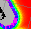
\includegraphics[width=0.75\textwidth]{images/costmap_2d_costgradient}
\caption{costmap\_2d sample \label{fig:costmap_2d_costgradient}}
\end{figure}

For obstacle mapping, the ROS navigation stack uses a software package called "costmap\_2d" \todo{reference to costmap2d wiki page}. This package takes in sensor information about the environment, builds a 2D or 3D fixed-resolution occupancy grid by raytracing that sensor information and inflates obstacles to facilitate navigation based on user provided robot parameters. For a visualization of a small portion of a costmap built from actual sensor data, see \autoref{fig:costmap_2d_costgradient}. In \autoref{fig:costmap_2d_costgradient} black pixels are the actual sensed obstacles, gray pixels are marked as "lethal" cost and the rest are a gradient between high cost in violet and low cost in red. Lethal cells are obstacles that have been inflated according the robot's geometry - specifically these are any cells that if the control point (or origin/center) of the robot were to enter one of these cells it would be in collision with the actual sensed obstacle. Outside of this inflated radius (also known as configuration space \todo{reference to configuration space}), the cost gradient expresses a preference for the path planners to stay away from obstacles unless other factors force the robot near to the obstacle.

While this approach works in many environments, there are downsides as well. Firstly, the fixed grid size

\begin{comment}
This will detail problems in ROS's Navigation stack when we last looked at it (and perhaps a discussion of how it has changed in the interim)

Outline:
	Mapping
		SimpleCostmap
		Fixed Grid size - needs changed for different environments and may affect trajectory scoring
		No option for temporal clearing of the map to reduce "leftovers" at small resolutions
	Local planning
		Scoring of trajectories
		Trajectories come from a fixed list of velocities and omegas (cross-product)
		simplistic cost function
		holonomic vs diff-drive
		scoring spin-in-place
	global planning
		dijkstra's planning
		replan only as a last resort
		may generate crappy plan since uses a circular robot with either inscribed or circumscribed radius
	localization
		defaults require tweaking for both map building and amcl
		amcl needs tuned to prevent "pops"
		
\end{comment}
